\documentclass{article}
\usepackage{tikz}
\usepackage{pgfplots}
\pgfplotsset{compat=1.18}
\usetikzlibrary{positioning, calc, arrows.meta, shapes.geometric, automata}
\begin{document}
\begin{figure}[h]\centering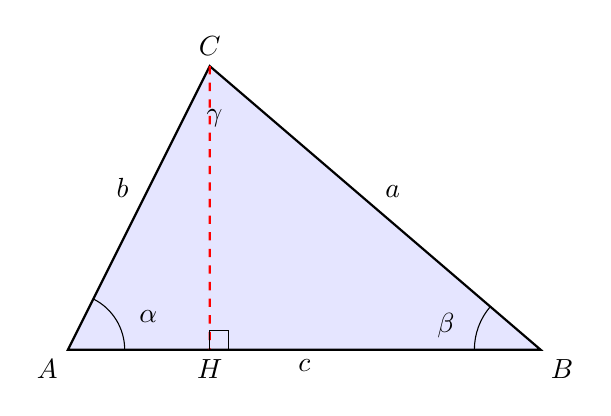
\begin{tikzpicture}[scale=1.2, thick]
  \coordinate (A) at (0,0);
  \coordinate (B) at (5,0);
  \coordinate (C) at (1.5,3);
  \draw[fill=blue!10] (A) -- (B) -- (C) -- cycle;
  % angle arcs
  \draw[thin] (A) ++(0.6,0) arc (0:63.4:0.6);
  \draw[thin] (B) ++(-0.7,0) arc (180:139.4:0.7);
  \node at (0.85,0.35) {$\alpha$};
  \node at (4.0,0.25) {$\beta$};
  \node at (1.55,2.45) {$\gamma$};
  % vertices and sides
  \node[below left] at (A) {$A$};
  \node[below right] at (B) {$B$};
  \node[above] at (C) {$C$};
  \node[below] at ($(A)!0.5!(B)$) {$c$};
  \node[above right] at ($(B)!0.5!(C)$) {$a$};
  \node[above left] at ($(A)!0.5!(C)$) {$b$};
  % altitude
  \draw[dashed, red] (C) -- (1.5,0) node[below, black] {$H$};
  \draw[thin] (1.5,0) rectangle +(0.2,0.2);
\end{tikzpicture}
\caption{Triangle with angles.}\end{figure}
\begin{figure}[h]\centering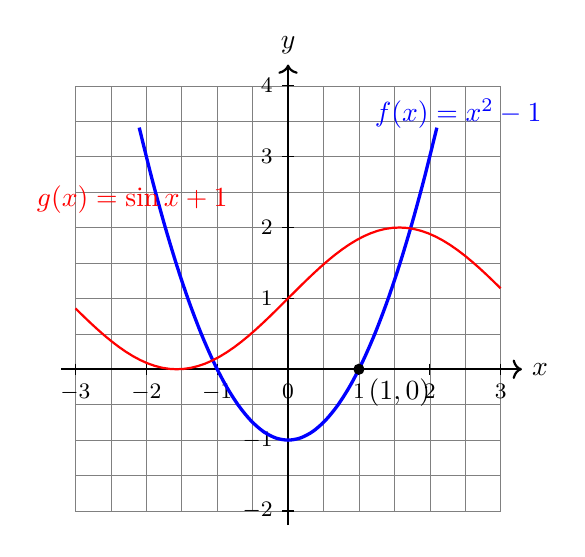
\begin{tikzpicture}[scale=0.9]
  \draw[help lines, step=0.5] (-3,-2) grid (3,4);
  \draw[->, thick] (-3.2,0) -- (3.3,0) node[right] {$x$};
  \draw[->, thick] (0,-2.2) -- (0,4.3) node[above] {$y$};
  \foreach \x in {-3,...,3} \draw (\x,0.08) -- (\x,-0.08) node[below] {\footnotesize $\x$};
  \foreach \y in {-2,-1,1,2,3,4} \draw (0.08,\y) -- (-0.08,\y) node[left] {\footnotesize $\y$};
  \draw[domain=-2.1:2.1, smooth, variable=\x, blue, very thick] plot ({\x}, {\x*\x - 1});
  \draw[domain=-3:3, samples=60, red, thick] plot (\x, {sin(\x r) + 1});
  \node[blue] at (2.4,3.6) {$f(x)=x^2-1$};
  \node[red] at (-2.2,2.4) {$g(x)=\sin x + 1$};
  \filldraw[black] (1,0) circle (2pt) node[below right] {$(1,0)$};
\end{tikzpicture}
\caption{Coordinate plane.}\end{figure}
\newpage
\begin{figure}[h]\centering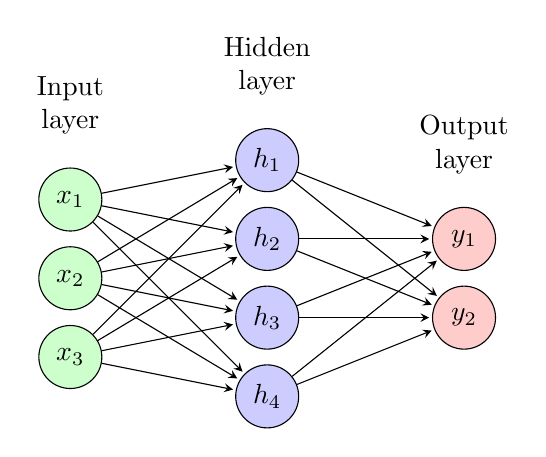
\begin{tikzpicture}[
  neuron/.style={circle, draw, minimum size=8mm, inner sep=0pt},
  input/.style={neuron, fill=green!20},
  hidden/.style={neuron, fill=blue!20},
  output/.style={neuron, fill=red!20},
  >=stealth, shorten >=1pt, node distance=2.2cm
]
  \foreach \i in {1,...,3}
    \node[input] (I\i) at (0,-\i) {$x_\i$};
  \foreach \j in {1,...,4}
    \node[hidden] (H\j) at (2.5,-\j+0.5) {$h_\j$};
  \foreach \k in {1,2}
    \node[output] (O\k) at (5,-\k-0.5) {$y_\k$};
  \foreach \i in {1,...,3}
    \foreach \j in {1,...,4}
      \draw[->] (I\i) -- (H\j);
  \foreach \j in {1,...,4}
    \foreach \k in {1,2}
      \draw[->] (H\j) -- (O\k);
  \node[above=0.3cm of I1, align=center] {Input\\layer};
  \node[above=0.3cm of H1, align=center] {Hidden\\layer};
  \node[above=0.3cm of O1, align=center] {Output\\layer};
\end{tikzpicture}
\caption{Neural network.}\end{figure}
\begin{figure}[h]\centering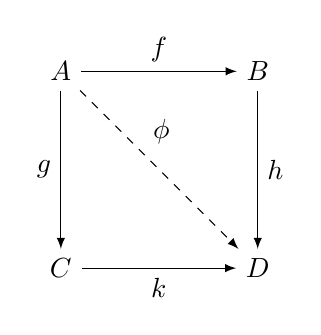
\begin{tikzpicture}[>=latex, node distance=2.5cm, auto]
  \node (A) {$A$};
  \node (B) [right of=A] {$B$};
  \node (C) [below of=A] {$C$};
  \node (D) [below of=B] {$D$};
  \draw[->] (A) to node {$f$} (B);
  \draw[->] (A) to node [swap] {$g$} (C);
  \draw[->] (B) to node {$h$} (D);
  \draw[->] (C) to node [swap] {$k$} (D);
  \draw[->, dashed] (A) to node[pos=0.4] {$\phi$} (D);
\end{tikzpicture}
\caption{Commutative diagram.}\end{figure}
\newpage
\begin{figure}[h]\centering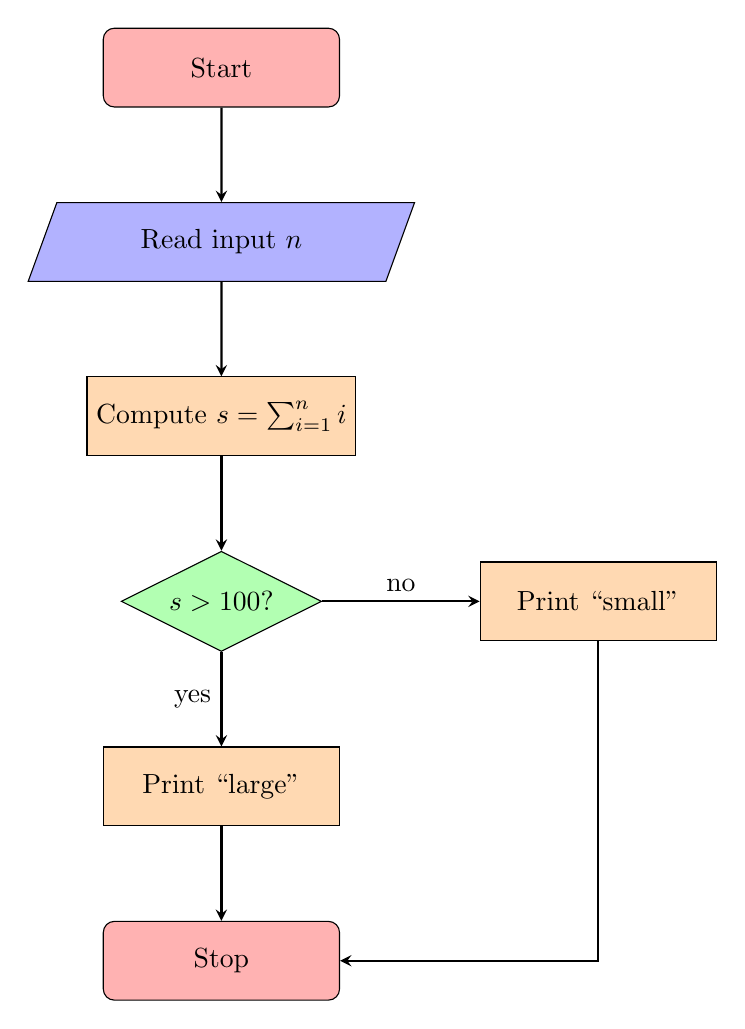
\begin{tikzpicture}[
  node distance=1.2cm and 2cm,
  startstop/.style={rectangle, rounded corners, minimum width=3cm, minimum height=1cm, text centered, draw=black, fill=red!30},
  process/.style={rectangle, minimum width=3cm, minimum height=1cm, text centered, draw=black, fill=orange!30},
  decision/.style={diamond, minimum width=2.5cm, minimum height=1cm, text centered, draw=black, fill=green!30, aspect=2},
  io/.style={trapezium, trapezium left angle=70, trapezium right angle=110, minimum width=3cm, minimum height=1cm, text centered, draw=black, fill=blue!30},
  arrow/.style={thick, ->, >=stealth}
]
  \node (start) [startstop] {Start};
  \node (in1) [io, below=of start] {Read input $n$};
  \node (pro1) [process, below=of in1] {Compute $s = \sum_{i=1}^n i$};
  \node (dec1) [decision, below=of pro1] {$s > 100$?};
  \node (pro2a) [process, below=of dec1] {Print ``large''};
  \node (pro2b) [process, right=of dec1] {Print ``small''};
  \node (stop) [startstop, below=of pro2a] {Stop};
  \draw [arrow] (start) -- (in1);
  \draw [arrow] (in1) -- (pro1);
  \draw [arrow] (pro1) -- (dec1);
  \draw [arrow] (dec1) -- node[anchor=east] {yes} (pro2a);
  \draw [arrow] (dec1) -- node[anchor=south] {no} (pro2b);
  \draw [arrow] (pro2b) |- (stop);
  \draw [arrow] (pro2a) -- (stop);
\end{tikzpicture}
\caption{Flowchart.}\end{figure}
\newpage
\begin{figure}[h]\centering\begin{tikzpicture}[auto, node distance=2cm, >=latex',
  block/.style={draw, fill=blue!10, rectangle, minimum height=3em, minimum width=6em},
  sum/.style={draw, fill=blue!10, circle, inner sep=0pt, minimum size=6mm},
  input/.style={coordinate}, output/.style={coordinate}]
  \node [input, name=input] {};
  \node [sum, right of=input] (sum) {$\Sigma$};
  \node [block, right of=sum, node distance=3cm] (controller) {Controller};
  \node [block, right of=controller, node distance=3.5cm] (system) {System};
  \draw [->] (controller) -- node[name=u] {$u$} (system);
  \node [output, right of=system, node distance=2.5cm] (output) {};
  \node [block, below of=u] (measurements) {Sensor};
  \draw [draw,->] (input) -- node {$r$} (sum);
  \draw [->] (sum) -- node {$e$} (controller);
  \draw [->] (system) -- node [name=y] {$y$}(output);
  \draw [->] (y) |- (measurements);
  \draw [->] (measurements) -| node[pos=0.99] {$-$} node [near end] {$y_m$} (sum);
\end{tikzpicture}
\caption{Block diagram.}\end{figure}
\begin{figure}[h]\centering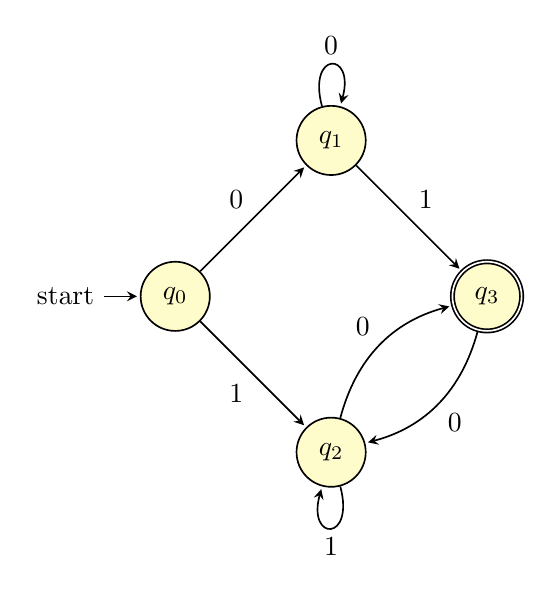
\begin{tikzpicture}[->, >=stealth, shorten >=1pt, auto, node distance=2.8cm, semithick]
  \tikzstyle{every state}=[fill=yellow!20, draw=black, text=black]
  \node[initial, state] (A) {$q_0$};
  \node[state] (B) [above right of=A] {$q_1$};
  \node[state] (D) [below right of=A] {$q_2$};
  \node[state, accepting] (C) [below right of=B] {$q_3$};
  \path (A) edge node {0} (B)
            edge node [swap] {1} (D)
        (B) edge [loop above] node {0} (B)
            edge node {1} (C)
        (C) edge [bend left] node {0} (D)
        (D) edge [loop below] node {1} (D)
            edge [bend left] node {0} (C);
\end{tikzpicture}
\caption{State machine.}\end{figure}
\newpage
\begin{figure}[h]\centering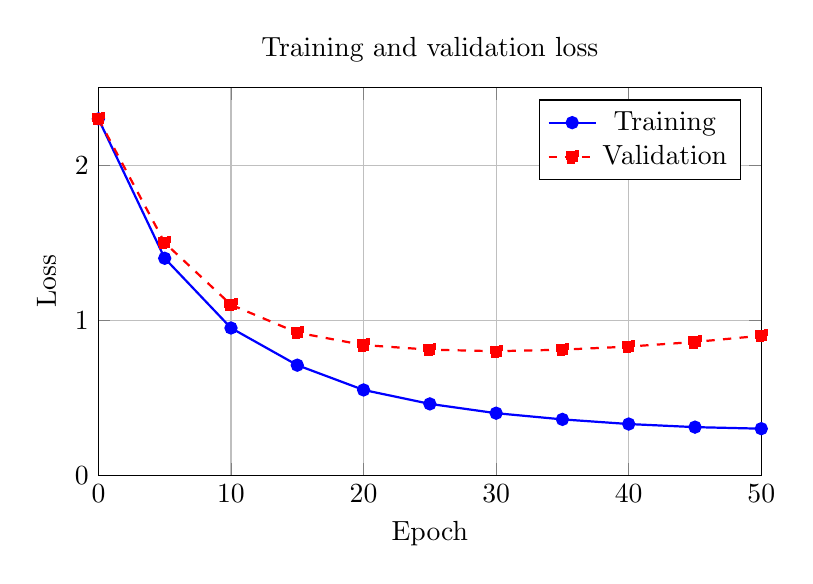
\begin{tikzpicture}
\begin{axis}[
    title={Training and validation loss},
    xlabel={Epoch},
    ylabel={Loss},
    xmin=0, xmax=50,
    ymin=0, ymax=2.5,
    legend pos=north east,
    grid=major,
    width=10cm, height=6.5cm,
]
\addplot[color=blue, mark=*, thick] coordinates {
    (0,2.3) (5,1.4) (10,0.95) (15,0.71) (20,0.55) (25,0.46) (30,0.40) (35,0.36) (40,0.33) (45,0.31) (50,0.30)
};
\addplot[color=red, mark=square*, thick, dashed] coordinates {
    (0,2.3) (5,1.5) (10,1.10) (15,0.92) (20,0.84) (25,0.81) (30,0.80) (35,0.81) (40,0.83) (45,0.86) (50,0.90)
};
\legend{Training, Validation}
\end{axis}
\end{tikzpicture}
\caption{Line plot.}\end{figure}
\begin{figure}[h]\centering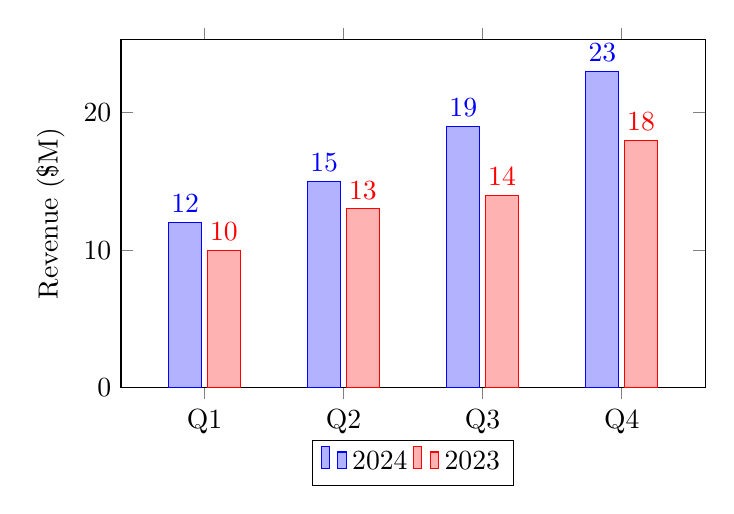
\begin{tikzpicture}
\begin{axis}[
    ybar,
    bar width=12pt,
    enlarge x limits=0.2,
    ymin=0,
    ylabel={Revenue (\$M)},
    symbolic x coords={Q1,Q2,Q3,Q4},
    xtick=data,
    nodes near coords,
    legend style={at={(0.5,-0.15)}, anchor=north, legend columns=-1},
    width=9cm, height=6cm,
]
\addplot coordinates {(Q1,12) (Q2,15) (Q3,19) (Q4,23)};
\addplot coordinates {(Q1,10) (Q2,13) (Q3,14) (Q4,18)};
\legend{2024, 2023}
\end{axis}
\end{tikzpicture}
\caption{Bar chart.}\end{figure}
\newpage
\begin{figure}[h]\centering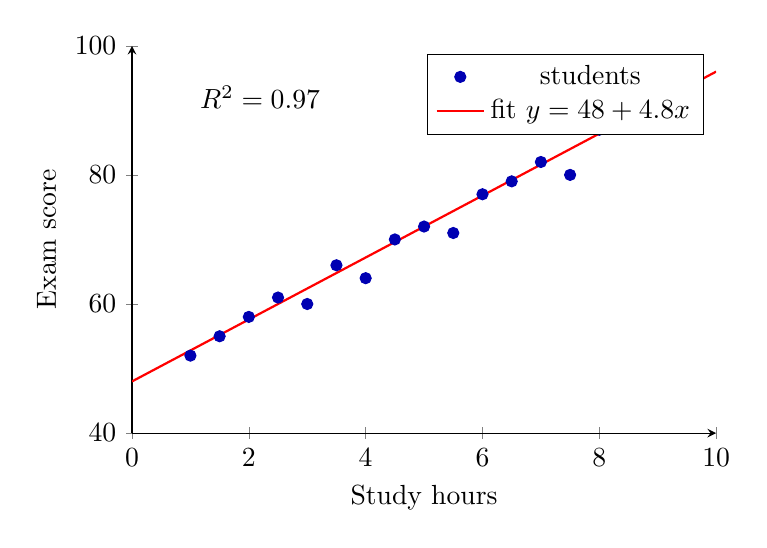
\begin{tikzpicture}
\begin{axis}[
    xlabel={Study hours},
    ylabel={Exam score},
    axis lines=left,
    xmin=0, xmax=10, ymin=40, ymax=100,
    width=9cm, height=6.5cm,
]
\addplot[only marks, mark=*, blue!70!black, mark size=2pt] coordinates {
  (1,52) (1.5,55) (2,58) (2.5,61) (3,60) (3.5,66) (4,64) (4.5,70) (5,72)
  (5.5,71) (6,77) (6.5,79) (7,82) (7.5,80) (8,87) (8.5,88) (9,91) (9.5,94)
};
\addplot[red, thick, domain=0:10] {48 + 4.8*x};
\addlegendentry{students}
\addlegendentry{fit $y = 48 + 4.8x$}
\node[anchor=west] at (axis cs:1,92) {$R^2 = 0.97$};
\end{axis}
\end{tikzpicture}
\caption{Scatter plot.}\end{figure}
\end{document}
